%\documentclass[12pt,handout]{beamer}
\documentclass[xcolor=dvipsnames,presentation]{beamer}
\usepackage{../oop-slides-lab}
\usepackage{soul}
\setbeamertemplate{bibliography item}[text]

\newcommand{\lab}{Lab10}

\title[{\lab} -- JavaFX]{Introduzione a JavaFX}

\date[\today]{\today}

\begin{document}

\frame[label=coverpage]{\titlepage}

%====================
%Outline
%====================
\begin{frame}<beamer>
 	\frametitle{Outline}
 	\tableofcontents[]
\end{frame}

%\section{Preparazione dell'ambiente di lavoro}

%\begin{frame}{Preparazione dell'ambiente di lavoro}
%	\begin{enumerate}\itemsep20pt
%		\item Clonare il repository degli esercizi
%		\begin{itemize}
%			\item \url{https://bitbucket.org/danysk/courses-2018-oop-lab-10}
%		\begin{itemize}
%		\item Opzionalmente, si fork-i il repository
%		\end{itemize}
%			\item Si copi la URI con cui effettuare il clone dall'interfaccia web di Bitbucket
%		\end{itemize}
%		\item Importare il repository in Eclipse come progetto Java
%		\item Configurare correttamente Eclipse, abilitare e configurare i plugin per il controllo di qualità del codice
%	\end{enumerate}
%\end{frame}
%
%\begin{frame}{Modalità di lavoro}
%	\begin{enumerate}
%		\item Seguire le istruzioni del file README.md nella root del repository
%		\item Tentare di capire l'esercizio in autonomia
%		\begin{itemize}
%			\item Contattare il docente se qualcosa non è chiaro
%		\end{itemize}
%		\item Risolvere l'esercizio in autonomia
%		\begin{itemize}
%			\item Contattare il docente se si rimane bloccati
%		\end{itemize}
%		\item Utilizzare le funzioni di test per verificare la soluzione realizzata
%		\item Cercare di risolvere autonomamente eventuali piccoli problemi che possono verificarsi durante lo svolgimento degli esercizi
%		\begin{itemize}
%			\item Contattare il docente se, anche \textbf{dopo aver usato il debugger}, non si è riusciti a risalire all'origine del problema
%		\end{itemize}
%		\item Scrivere la Javadoc per l'esercizio svolto
%		\item Assicurarsi che non ci siano warning nel proprio codice
%		\item Effettuare \textit{almeno} un commit ad esercizio completato
%		\item \textbf{A esercizio ultimato sottoporre la soluzione al docente}
%		\item Proseguire con l'esercizio seguente
%	\end{enumerate}
%\end{frame}
%
%\section{Swing Toolkit (richiami)}
%
%\begin{frame}{GUI in Java: Swing Toolkit}
%\begin{itemize}\itemsep10pt
%\item Sviluppato per fornire un insieme di componenti per la realizzazione di GUI, più completi e sofisticati rispetto a quelli presenti in AWT (Abstract Window Toolkit)
%\begin{itemize}
%\item Oltre ai componenti già presenti in AWT, ne propone di nuovi: es. Tabbed Panel, Lists, etc.
%\item Tutti i componenti di swing sono sviluppati in Java (in AWT si utilizza codice nativo) e sono quindi platform-independent (\textit{Lightweight UI})
%\end{itemize}
%\item Propone un proprio look-and-feel per le applicazioni desktop
%\begin{itemize}
%\item Supporta anche i pluggable look-and-feel
%\end{itemize}
%\item Ha un'architettura basata sul pattern MVC e segue un modello di programmazione single-thread
%\end{itemize}
%\end{frame}

\section{Java Swing: Richiami}

\begin{frame}{Event Dispatch Thread (EDT) in Swing}
\begin{itemize}\itemsep10pt
\item E' il thread deputato alla gestione degli eventi della GUI di un'applicazione Swing-based
\item Avviato dalla JVM alla creazione del primo JFrame
\begin{itemize}
\item (nota) L'applicazione non termina al completamento del main
\end{itemize}
\item Tutti gli eventi relativi a componenti della GUI sono demandati all'EDT
\begin{itemize}
\item Ciascun evento è gestito a condizione che la gestione di tutti quelli precedenti sia terminata
\item Si presuppone che la gestione di ciascun evento non implichi una situazione di \emph{stallo} dell'applicazione (dell'EDT)
\end{itemize}
\item \textbf{Swing non è thread-safe!}
\begin{itemize}
\item Si presuppone che l'EDT sia l'unico thread ad eccedere alla GUI
\item Si utilizza la libreria \texttt{SwingUtilities} -- i metodi \texttt{invokeLater()} and \texttt{invokeAndWait()} -- per accedere alla GUI da altri thread
\end{itemize}
\end{itemize}
\end{frame}

\begin{frame}{Limiti (e svantaggi) di Swing}
\begin{itemize}\itemsep10pt
\item L'insieme dei componenti offerti è piuttosto limitato
\begin{itemize}
\item \dots se non altro, per le applicazioni moderne
\item \dots il look-and-feel è old-style
\item \dots non supportano (tutte) le nuove interfacce touch screen
\end{itemize}
\item La gestione dello z-level tra i componenti non è banale
\item Non supporta forme di validazione per i dati nei componenti di input
\item Non propone alcun supporto nativo per la gestione del 3D
\item Ha il limite (e la problematica) della non thread-safeness
\item Non è possibile separare il controller dalla relativa view per i componenti Swing preesistenti
\end{itemize}
\end{frame}

\section{Introduzione a JavaFX}

\begin{frame}{JavaFX}
\begin{itemize}\itemsep20pt
\item Libreria Java per la creazione di GUI per Rich Applications multi-piattaforma
\begin{itemize}
\item Disponibile dal 2008 (v. 1.0 -- 2.2) come libreria stand-alone
\item Presente ``\emph{stabilmente}'' nel JDK da Java 8 (v. JavaFX 8)
\item \st{Introdotto ufficialmente in Java con l'idea di sostituire (gradualmente) Swing}
\item Torna ad essere una libreria stand-alone da Java 11:
 è opensource e parte del progetto OpenJDK -- \url{https://openjfx.io}
\end{itemize}
\item Propone un look-and-feel personalizzabile
\begin{itemize}
\item La descrizione dello stile/aspetto dei componenti della GUI è separato dalla relativa implementazione
\item Segue il pattern MVC
\end{itemize}
\item Consente la creazione di GUI moderne, di qualità e ben adattabili a qualunque piattaforma e supporto hardware
\end{itemize}
\end{frame}

%\begin{frame}{JavaFX (dal 2018)}
%
%\begin{block}{Java Client Roadmap Update (Oracle White Paper, March 2018)}
%\begin{small}
%\begin{center}
%\emph{Over the last decade, the JavaFX technology has found its niche where it enjoys the support of a developer community. At the same time, the magnitude of opportunities for cross-platform toolkits [...] has been eroded by the rise of ``mobile first'' and ``web first'' apps.}
%\begin{tiny}
%\url{https://www.oracle.com/technetwork/java/javase/javaclientroadmapupdate2018mar-4414431.pdf}
%\end{tiny}
%\end{center}
%\end{small}
%\end{block}
%%
%\begin{itemize}
%\item Pertanto:
%\begin{itemize}
%\item JavaFX continuerà ad essere supportato fino al 2022 da Oracle (solo nel JDK 8)
%\item JavaFX sara disponibile come libreria esterna opensource (affidata ad OpenJDK) -- \url{https://openjfx.io}
%\end{itemize}
%\end{itemize}
%\end{frame}

%\begin{frame}{JavaFX 11}
%\begin{itemize}\itemsep10pt
%\item Al momento, si tratta del porting as-is di JavaFX 8 sul JDK 11
%\begin{itemize}
%\item Unica novità significativa, FX Robot API per la simulazione dell'interazione dell'utente con la GUI
%\end{itemize}
%\item Implica l'utilizzo del JDK 11
%\item Risente ancora di molti bug
%\begin{itemize}
%\item \url{https://github.com/javafxports/openjdk-jfx/blob/jfx-11/doc-files/release-notes-11.0.1.md\#release-notes-for-javafx-1101}
%\end{itemize}
%\end{itemize}
%\end{frame}

\subsection{Architettura e Key Features}

\begin{frame}{JavaFX: Key Features (1/2)}
\begin{block}{Java APIs}
\begin{itemize}
\item Libreria che include classi e interfacce scritte in Java %e compilato con retro compatibilità fino a Java 7
\item Nel 2020, la versione più recente, JavaFX 15, richiede JDK $\geq$ 11
\end{itemize}
\end{block}
%
\begin{block}{FXML}
\begin{itemize}
\item FXML è un linguaggio dichiarativo per definire la GUI di un'applicazione JavaFX-based
\item Il suo impiego non è indispensabile, ma fortemente consigliato per una buona \emph{separation of concerns}
\end{itemize}
\end{block}
%
\begin{block}{Interoperabilità con Swing}
\begin{itemize}
\item GUI Swing esistenti possono includere componenti JavaFX (cf. \texttt{JFXPanel})
\item E' possibile inserire componenti Swing in interfacce JavaFX (cf. \texttt{SwingNode})
\end{itemize}
\end{block}
\end{frame}

\begin{frame}{JavaFX: Key Features (2/2)}
\begin{block}{Graphics API}
\begin{itemize}
\item Supporto nativo per la grafica 3D
\item Abilita la possibilità di disegnare direttamente sulla superficie (canvas) dell'applicazione
\end{itemize}
\end{block}
%
\begin{block}{Supporto per schermi Multi-touch e Hi-DPI}
\begin{itemize}
\item Fornisce il supporto per funzionalità  multi-touch, in funzione della piattaforma in cui l'applicazione è in esecuzione
\item Garantisce una buona visualizzazione della GUI anche su schermi ad alta densità
\end{itemize}
\end{block}
\end{frame}

%\begin{frame}{JavaFX: Architettura}
%\begin{figure}
%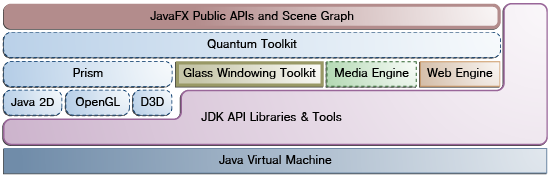
\includegraphics[width=0.95\textwidth]{img/javafx-architecture.png}
%\end{figure}
%\begin{itemize}
%\item \emph{per approfondimenti} -- \url{https://docs.oracle.com/javase/8/javafx/get-started-tutorial/jfx-architecture.htm}
%\end{itemize}
%\end{frame}

\subsection{Key Concepts}

\begin{frame}{Elementi fondamentali (1/3)}
\begin{block}{Stage}
\begin{itemize}
\item Il contenitore (esterno) dove la GUI sarà visualizzata
\begin{itemize}
\item es. una finestra del S.O.
\item Equivalente al \texttt{JFrame} di Swing
\item Non è compito del programmatore creare una sua istanza.
\end{itemize}
\item \url{https://openjfx.io/javadoc/15/javafx.graphics/javafx/stage/Stage.html}
\end{itemize}
\end{block}

\begin{block}{Scene}
\begin{itemize}
\item Rappresenta il contenuto di uno Stage (una \emph{pagina} della GUI)
\begin{itemize}
\item ogni Stage può avere più istanze diverse di Scene
\end{itemize}
\item Di fatto, è un container di Node(s)
\item \url{https://openjfx.io/javadoc/15/javafx.graphics/javafx/scene/Scene.html}
\end{itemize}
\end{block}
\end{frame}

\begin{frame}[fragile]{Applicazione JavaFX: GUI vuota}

\begin{itemize}
\item \texttt{Application}: entry point of a JavaFX application
\\ \url{https://openjfx.io/javadoc/15/javafx.graphics/javafx/application/Application.html}
\end{itemize}

\begin{lstlisting}
public class Main extends javafx.application.Application {

	@Override
	public void start(Stage stage) throws Exception {
		Group root = new Group();
		Scene scene = new Scene(root, 500, 300);
		stage.setTitle("JavaFX Demo");
		stage.setScene(scene);
		stage.show();
	}

	public static void main(String[] args) { launch(args); }
}
\end{lstlisting}
\end{frame}

\begin{frame} {Elementi fondamentali (2/3)}
\begin{block}{Node(s)}
\begin{itemize}
\item Un elemento/componente della scena
\begin{itemize}
\item Ciascun nodo ha sia la parte di view (aspetto) sia la parte di controller (comportamento)
\item Hanno proprietà e possono generare eventi
\end{itemize}
\item Possono essere organizzati gerarchicamente
\item \url{https://openjfx.io/javadoc/15/javafx.graphics/javafx/scene/Node.html}
\end{itemize}
\end{block}
\end{frame}

\begin{frame}{Elementi fondamentali (3/3)}
\begin{figure}
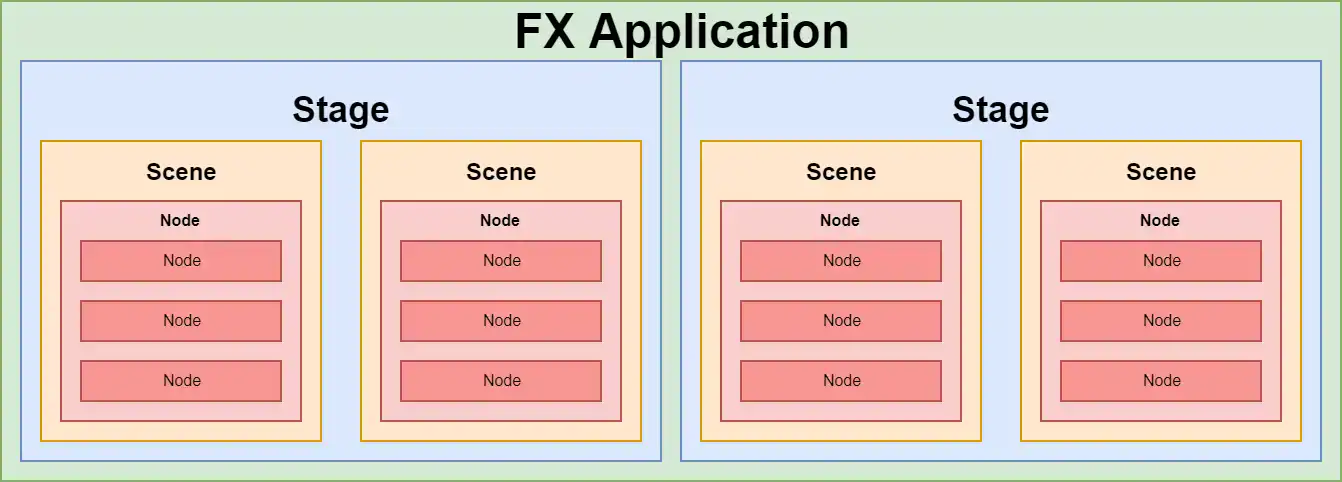
\includegraphics[width=\textwidth]{img/javafx-app.png}
\end{figure}
\end{frame}

%\begin{frame}{Nodes Hiearchy}
%
%\end{frame}

\begin{frame}{Struttura di un'applicazione JavaFX-based}
\begin{figure}
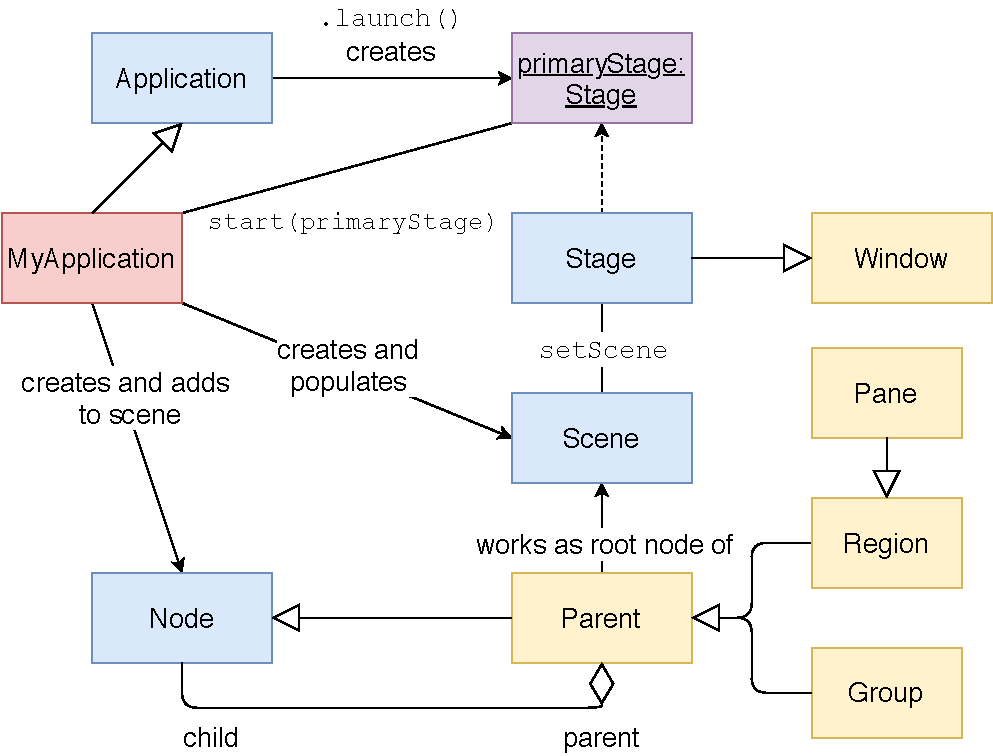
\includegraphics[height=0.86\textheight]{img/javafx-app-structure.pdf}
\end{figure}
\end{frame}

\begin{frame}{Linee guida}
\begin{enumerate}\itemsep20pt
\item La classe principale di un'applicazione JavaFX deve estendere la classe \texttt{javafx.application.Application}
\item Il metodo \texttt{main()} deve chiamare il metodo \texttt{launch()}
\begin{itemize}
\item Si tratta di un metodo statico della classe \texttt{Application}
\end{itemize}
\item Il metodo \texttt{void start(Stage primaryStage)} è, di fatto, l'entry point dell'applicazione JavaFX (lo stage primario è creato dalla piattaforma)
\item La scena definita per lo stage (vedi metodo \texttt{setScene()}) costituisce il container principale per tutti i componenti della GUI
\end{enumerate}
\end{frame}

\begin{frame}{Nodi e Proprietà}
\begin{itemize}\itemsep10pt
\item Ogni scena può essere popolata con una gerarchia di nodi
\item Ciascun nodo (componente) espone diverse proprietà
\begin{itemize}
\item relative all'aspetto (es. \texttt{size}, \texttt{posizion}, \texttt{color}, \dots)
\item relative al contenuto (es. \texttt{text}, \texttt{value}, \dots)
\item relative al comportamento (es. \texttt{event handlers}, \texttt{controller}, \dots)
\end{itemize}
\item Ciascun nodo genera eventi in relazione ad azioni dell'utente
\end{itemize}
\end{frame}

\begin{frame}[fragile]{GUI con bottone e label}
\begin{lstlisting}
public class Example1 extends Application{
	@Override
	public void start(Stage stage) throws Exception {
		Label lbl = new Label();
		lbl.setText("Label text here...");

		Button btn = new Button();
		btn.setText("Click me");

		HBox root = new HBox();
		root.getChildren().add(btn);
		root.getChildren().add(lbl);

		stage.setTitle("JavaFX - Example 1");
		stage.setScene(new Scene(root, 300,250));
		stage.show();
	}

	public static void main(String[] args) { launch(args); }
}
\end{lstlisting}
\end{frame}

\begin{frame}{Layouts (1/2)}
\begin{block}{Group}
\begin{itemize}
\item Non impone nessun posizionamento per i componenti figli
\item Da utilizzare per posizionare i componenti figli in posizioni fisse
\end{itemize}
\end{block}

\begin{block}{Region}
\begin{itemize}
\item Tutte le sue specializzazioni forniscono diversi layout general purpose
\item Sono simili a quelli offerti da Swing
\end{itemize}
\end{block}

\begin{block}{Control}
\begin{itemize}
\item Costituisce l'insieme dei layout personalizzabili
\item Ciascun layout di questo tipo fornisce specifiche API per l'aggiunta dei componenti figli
\end{itemize}
\end{block}
\url{https://openjfx.io/javadoc/13/javafx.graphics/javafx/scene/layout/package-summary.html}
\end{frame}

\begin{frame}{Layouts (2/2)}
\begin{figure}
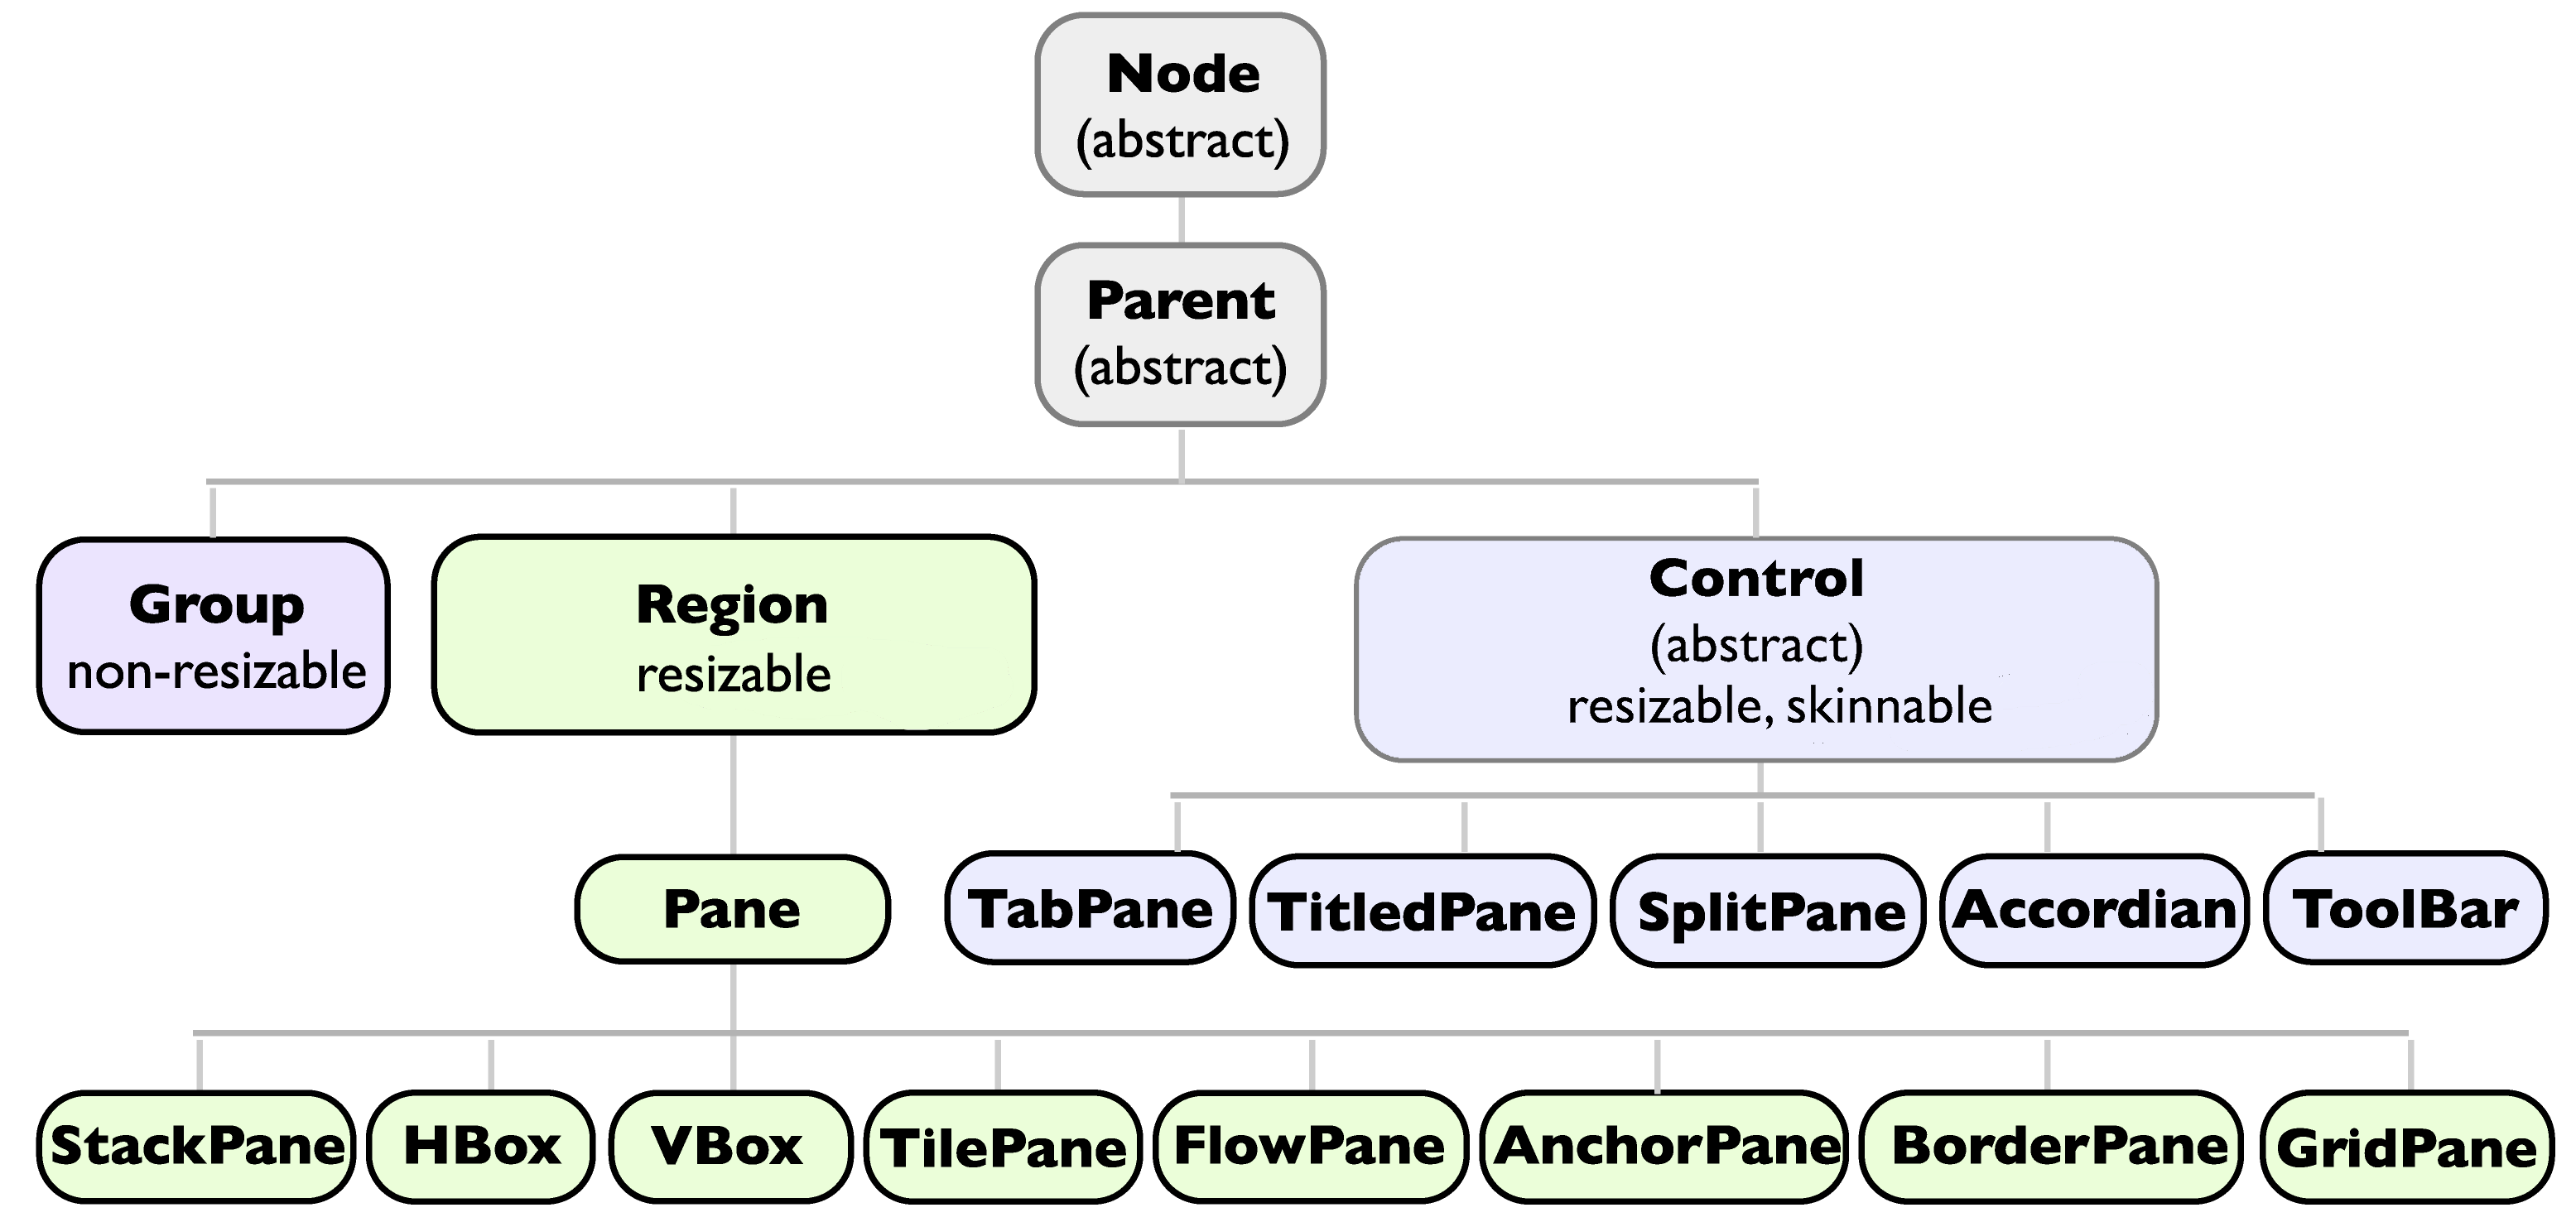
\includegraphics[width=0.75\textwidth]{img/layouts.png}
\end{figure}

\begin{block}{Aggiungere componenti ad un layout}
\begin{itemize}
\item Il metodo \texttt{ObservableList<Node> getChildren()} restituisce la lista di nodi figli di un qualunque nodo/layout
\item Alla lista possono essere aggiunti (\texttt{boolean add(Node e)}) e gestiti i componenti figli
\end{itemize}
\end{block}
\end{frame}

\begin{frame}[fragile]{Eventi}
\begin{itemize}\itemsep10pt
\item Possono essere generati in relazione nodi e alle scene
\begin{itemize}
\item Fanno riferimento alla classe \texttt{javafx.event.Event}
\end{itemize}
\item Come in swing, si generano in funzione di azioni dell'utente sulla GUI
\item Possono essere gestiti attraverso \emph{event handlers} (devono implementare l'interfaccia \texttt{EventHandler})
\item Ogni nodo può registrare uno o più event handlers
\begin{itemize}
\item In generale, attraverso i metodi \texttt{setOn...}()
\item Ogni event handler deve implementare il metodo \texttt{void handle(ActionEvent e)}
\end{itemize}
\end{itemize}

\begin{block}{Es. Gestione del click su un Button Node}
\begin{lstlisting}
btn.setOnMouseClicked(event -> {
 lbl.setText("Hello, JavaFX World!");
});
\end{lstlisting}
\end{block}
\end{frame}

\begin{frame}[fragile]{Esempio con più Stage (1/2)}
\begin{lstlisting}[basicstyle=\tiny]
public class Main extends Application {

  @Override
  public final void start(final Stage mainStage) {
    final Scene scene = new Scene(initSceneUI());
    mainStage.setScene(scene);
    mainStage.setTitle("JavaFX Example");
    mainStage.show();
  }

  private Parent initSceneUI() {
    final Label inputLbl = new Label("Input: ");
    final TextField inputArea = new TextField();
    final Button okBtn = new Button("Open a new Stage with the input data!");

    okBtn.setOnMouseClicked(event -> {
      new SecondStage(inputArea.getText()).show();
    });

    final BorderPane root = new BorderPane();
    root.setRight(okBtn);
    root.setLeft(inputLbl);
    root.setCenter(inputArea);

    BorderPane.setAlignment(inputLbl, Pos.CENTER_LEFT);
    BorderPane.setAlignment(okBtn, Pos.CENTER_RIGHT);

    return root;
  }

  public static void main(final String[] args) { launch(args); }
}
\end{lstlisting}
\end{frame}

\begin{frame}[fragile]{Esempio con più Stage (2/2)}
\begin{lstlisting}[basicstyle=\tiny]
public class SecondStage extends Stage {
  private Label lbl;

  public SecondStage(final String message) {
    super();

	setTitle("New Window...");

	setScene(new Scene(initSceneUI(), 400, 200));

	lbl.setText(message);
  }

  private Parent initSceneUI() {
    lbl = new Label();

	FlowPane root = new FlowPane();
	root.setAlignment(Pos.CENTER);

	root.getChildren().add(lbl);

	return root;
  }
}
\end{lstlisting}
\end{frame}



\section{FXML}

\begin{frame}{Separazioni di ruoli e contenuti}
\begin{itemize}\itemsep10pt
\item In JavaFX è possibile separare il design della GUI dal codice sorgente che la riguarda
\item Il design della GUI può essere descritto attraverso un linguaggio di markup denominato FXML
\end{itemize}
\begin{figure}
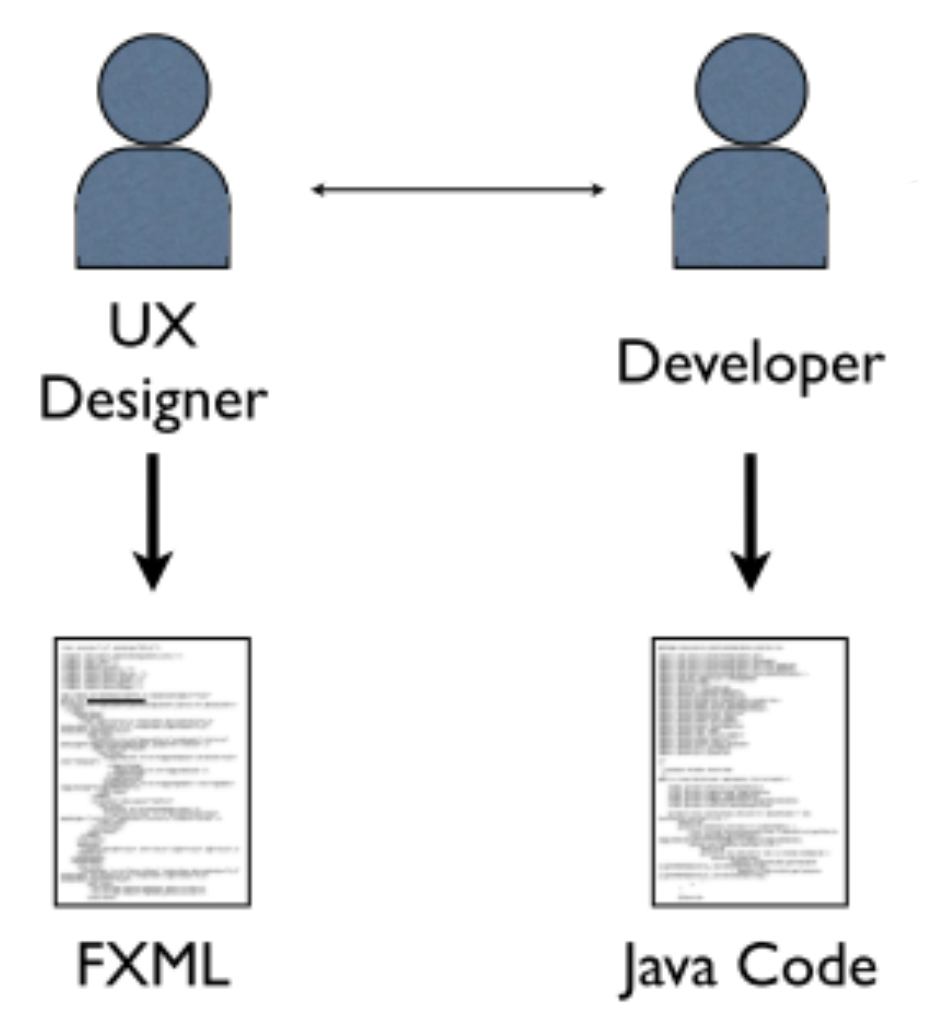
\includegraphics[width=0.4\textwidth]{img/soc.png}
\end{figure}
\end{frame}

\begin{frame}{FXML}
\begin{itemize}\itemsep20pt
\item Linguaggio di markup basato su XML
\item Descrive la struttura della GUI
\begin{itemize}
\item Tutti i componenti della GUI sono specificati mediante tag specifici
\item Le proprietà sono specificate come attributi su ciascun tag, nella forma chiave-valore
\end{itemize}
\item Ogni file FXML (con estensione \texttt{.fxml}) deve essere un file XML valido
\begin{itemize}
\item Deve iniziare con il tag: \texttt{<?xml version="1.0" encoding="UTF-8"?>}
\end{itemize}
\end{itemize}
\end{frame}

\begin{frame}[fragile]{Esempio di GUI in FXML}
\begin{lstlisting}
<?xml version="1.0" encoding="UTF-8"?>

<?import javafx.scene.control.*?>
<?import javafx.scene.layout.*?>

<VBox xmlns="http://javafx.com/javafx" xmlns:fx="http://javafx.com/fxml">
  <children>
    <Button fx:id="btn"
    	alignment="CENTER"
    	text="Say Hello!"
    	textAlignment="CENTER" />

    <Label fx:id="lbl"
    	alignment="CENTER_LEFT"
    	text="Label Text Here!"
    	textAlignment="LEFT" />
  </children>
</VBox>
\end{lstlisting}
\end{frame}

\begin{frame}[fragile]{Esempio di GUI in FXML -- Note}
\begin{enumerate}\itemsep15pt
\item Attraverso il tag \texttt{<?import ... ?>} è possibile specificare i package in cui recuperare le classi dei componenti d'interesse
\begin{itemize}
\item E' equivalente all'\texttt{import} di Java
\end{itemize}
\item Il container principale (unico per il singolo file) \underline{deve} specificare gli attributi \texttt{xmlns} e \texttt{xmlns:fx}
\begin{itemize}
\item \begin{verbatim}xmlns="http://javafx.com/javafx"\end{verbatim}
\item \begin{verbatim}xmlns:fx="http://javafx.com/fxml"\end{verbatim}
\end{itemize}
\item Ogni container deve specificare i nodi figli all'interno dei tag \texttt{$<$children$>$} e \texttt{$<$/children$>$}
\item Ogni nodo deve definire il proprio ID mediante l'attributo \texttt{fx:id}
\begin{itemize}
\item Es. \texttt{$<$TextField fx:id="textField1"/$>$}
\end{itemize}
\end{enumerate}
\end{frame}

\begin{frame}[fragile]{Collegare il design della GUI al codice Java}
\begin{itemize}\itemsep10pt
\item La GUI descritta nel file FXML deve essere collegata alla scena agganciata allo stage dell'applicazione
\item Si può utilizzare il componente \texttt{javafx.fxml.FXMLLoader}
\begin{itemize}
\item Il metodo statico \texttt{load(URL location)}
\end{itemize}
\item Nota: occorre dichiarare il modulo \texttt{javafx.fxml} (si veda ad es. la build Gradle più avanti)
\end{itemize}
\begin{block}{FXMLLoader (esempio)}
\begin{itemize}
\item Si suppone che nel progetto sia presente il file \texttt{main.fxml} contenente una descrizione valida per la GUI da caricare
\end{itemize}
\begin{lstlisting}
Parent root = FXMLLoader.load(ClassLoader.getSystemResource("layouts/main.fxml"));
\end{lstlisting}
\end{block}
\end{frame}

\begin{frame}[fragile]{FXMLLoader (esempio completo)}
\begin{lstlisting}
public class Example3 extends Application{

	@Override
	public void start(Stage stage) throws Exception {
Parent root = FXMLLoader.load(ClassLoader.getSystemResource("layouts/main.fxml"));

		Scene scene = new Scene(root, 500, 250);

		stage.setTitle("JavaFX - Example 3");
		stage.setScene(scene);
		stage.show();
	}

	public static void main(String[] args) {
		launch(args);
	}
}
\end{lstlisting}
\end{frame}

\begin{frame}[fragile]{Lookup dei componenti della GUI}
\begin{itemize}
\item Il riferimento ai componenti (nodi) inseriti nella GUI definita nel file FXML può essere recuperato tramite la scena a cui la GUI è stata collegata
\begin{itemize}
\item Metodo \texttt{Node lookup(String id)}
\end{itemize}

\begin{block}{Node Lookup (esempio)}
\begin{lstlisting}
Label lbl = (Label) scene.lookup("#lbl");

Button btn = (Button) scene.lookup("#btn");
btn.setOnMouseClicked(handler -> {
	lbl.setText("Hello, FXML!");
});
\end{lstlisting}
\end{block}
\item \textbf{Attenzione}: il metodo \texttt{lookup} richiede come parametro l'id specificato per il componente (attributo \texttt{fx:id} nel file FXML) preceduto dal simbolo \#
\end{itemize}
\end{frame}

\begin{frame}{GUI Controller e Node Injection}
\begin{itemize}\itemsep20pt
\item Per una corretta separazione dei contenuti (e una buona implementazione del pattern MVC in JavaFX) è opportuno specificare un oggetto \emph{controller} per ciascuna GUI
\begin{itemize}
\item Il parent component della GUI deve definire l'attributo \texttt{fx:controller} con valore riferito al percorso completo della classe che fungerà da controller
\end{itemize}
\item Mediante l'annotazione \texttt{@FXML} è possibile recuperare:
\begin{itemize}
\item I riferimenti ai vari nodi (senza utilizzare il meccanismo di lookup)
\item Associare gli event handler ai vari eventi dei componenti
\end{itemize}
\end{itemize}
\end{frame}

\begin{frame}[fragile]{Esempio Completo (1/3) -- Application}
\begin{lstlisting}
public class CompleteExample extends Application{

	@Override
	public void start(Stage stage) throws Exception {
		VBox root = FXMLLoader.load(ClassLoader.getSystemResource("layouts/main.fxml"));

		Scene scene = new Scene(root, 500, 250);

		stage.setTitle("JavaFX - Complete Example");
		stage.setScene(scene);
		stage.show();
	}

	public static void main(String[] args) {
		launch(args);
	}
}
\end{lstlisting}
\end{frame}

\begin{frame}[fragile]{Esempio Completo (2/3) -- GUI (FXML file)}
\begin{lstlisting}
<?xml version="1.0" encoding="UTF-8"?>

<?import javafx.scene.control.*?>
<?import javafx.scene.layout.*?>

<VBox
    xmlns="http://javafx.com/javafx"
    xmlns:fx="http://javafx.com/fxml"
	fx:controller="it.unibo.oop.lab.javafx.UIController">
  <children>
    <Button fx:id="btn"
    	alignment="CENTER"
    	text="Say Hello!"
    	onMouseClicked="#btnOnClickHandler" />

    <Label fx:id="lbl"
    	alignment="CENTER_LEFT"
    	text="Label Text Here!" />
  </children>
</VBox>
\end{lstlisting}
\end{frame}

\begin{frame}[fragile]{Esempio Completo (3/3) -- GUI Controller}
\begin{lstlisting}
public class UIController {

	@FXML
	private Label lbl;

	@FXML
	private Button btn;

	@FXML
	public void btnOnClickHandler() {
		lbl.setText("Hello, World!");
	}
}
\end{lstlisting}
\end{frame}

\section{Integrazione JavaFX e Swing}

\begin{frame}{Integrare JavaFX e Swing}
\begin{itemize}
\item L'integrazione può avvenire nelle due direzioni
	\iz{
	\item Si possono includere elementi Swing in applicazioni JavaFX attraverso \texttt{SwingNode}
	\item Si possono includere elementi JavaFX in applicazioni Swing attraverso \texttt{JFXPanel}
	\item Nota: \texttt{SwingNode} e \texttt{JFXPanel} si trovano nel modulo \texttt{javafx.swing}
	}
%\item In Java, un'applicazione può contenere sia GUI programmate in Swing, sia altre programmate in JavaFX
%\begin{itemize}
%\item La Main UI deve essere in Swing
%\item Si integrano Scene di JavaFX in JFrame avvalendosi di componenti che sono istanze di \texttt{JFXPanel}, eseguite nel thread specifico di JavaFX
%\end{itemize}
\item Va prestata particolare attenzione a dove viene eseguito il codice che gestisce la GUI
\begin{itemize}
\item \texttt{javafx.application.Platform.runLater()}, per eseguire codice nel thread dedicato a JavaFX
\item \texttt{javax.swing.SwingUtilities.invokeLater()}, per eseguire codice nel thread dedicato a Swing
\end{itemize}
\end{itemize}
\end{frame}

\begin{frame}[allowframebreaks,fragile]{Usare JavaFX in applicazioni Swing: esempio}

\begin{lstlisting}[basicstyle=\tiny]
public static void main(final String[] args){
  initMainJFrame(new JFrame("JFrame GUI"));
}
\end{lstlisting}

\begin{lstlisting}[basicstyle=\tiny]
private static void initMainJFrame(final JFrame frame) {
  final JButton button = new JButton();
  button.setText("Launch JavaFX Scene");
  button.addActionListener(event -> {
    final JFXPanel jfxPanel = new JFXPanel();
    Platform.runLater(() -> {
      jfxPanel.setScene(new Scene(initJavaFXSceneUI(), 300, 300));
      SwingUtilities.invokeLater(() -> {
        final JFrame frameWithJavaFX = new JFrame("JFrame with JavaFX embedded!");
        frameWithJavaFX.add(jfxPanel);
        frameWithJavaFX.pack();
        frameWithJavaFX.setVisible(true);
  }); }); });

  final JPanel panel = new JPanel();
  panel.setLayout(new FlowLayout());
  panel.add(button);

  frame.setContentPane(panel);
  frame.setSize(300, 300);
  frame.setDefaultCloseOperation(JFrame.EXIT_ON_CLOSE);
  frame.setVisible(true);
}
\end{lstlisting}

\begin{lstlisting}[basicstyle=\tiny]
private static Parent initJavaFXSceneUI() {
  final Label lbl = new Label();
  lbl.setText("Hello, JavaFX World!");

  final Button btn = new Button();
  btn.setText("Say Hello");
  btn.setOnMouseClicked(event -> {
    lbl.setText("Hello from Button!");
  });

  final VBox root = new VBox();
  root.getChildren().add(lbl);
  root.getChildren().add(btn);

  return root;
}
\end{lstlisting}

\end{frame}

\section{Utilizzo di JavaFX con Eclipse e Gradle}

%\subsection{JavaFX con JDK 8}
%
%\begin{frame}{JavaFX in Eclipse (JDK 8)}
%\begin{itemize}\itemsep20pt
%\item La libreria JavaFX è presente unicamente nel JDK 8
%\begin{itemize}
%\item Distribuita attraverso il file \texttt{jfxrt.jar} presente nella directory \texttt{/lib/ext} della propria installazione del JDK
%\end{itemize}
%\item Tutti le librerire \emph{esterne} \underline{non} sono automaticamente accessibili da tutti i progetti aperti nell'IDE Eclipse
%\begin{itemize}
%\item In realtà dipende dalla versione di Eclipse\dots
%\end{itemize}
%\item Deve essere definita una regola d'accesso per JavaFX in relazione allo specifico progetto Java aperto in Eclipse
%\end{itemize}
%\end{frame}
%
%\begin{frame}{Configurazione del progetto (1/2)}
%\begin{itemize}
%\item (tasto DX sul progetto) $>$ Properties $>$ Java Build Path
%\item (tab Libraries) $>$ Click sul JRE System Library $>$ Selezionare \textit{Access rules} $>$ Click su Edit
%\end{itemize}
%\begin{figure}
%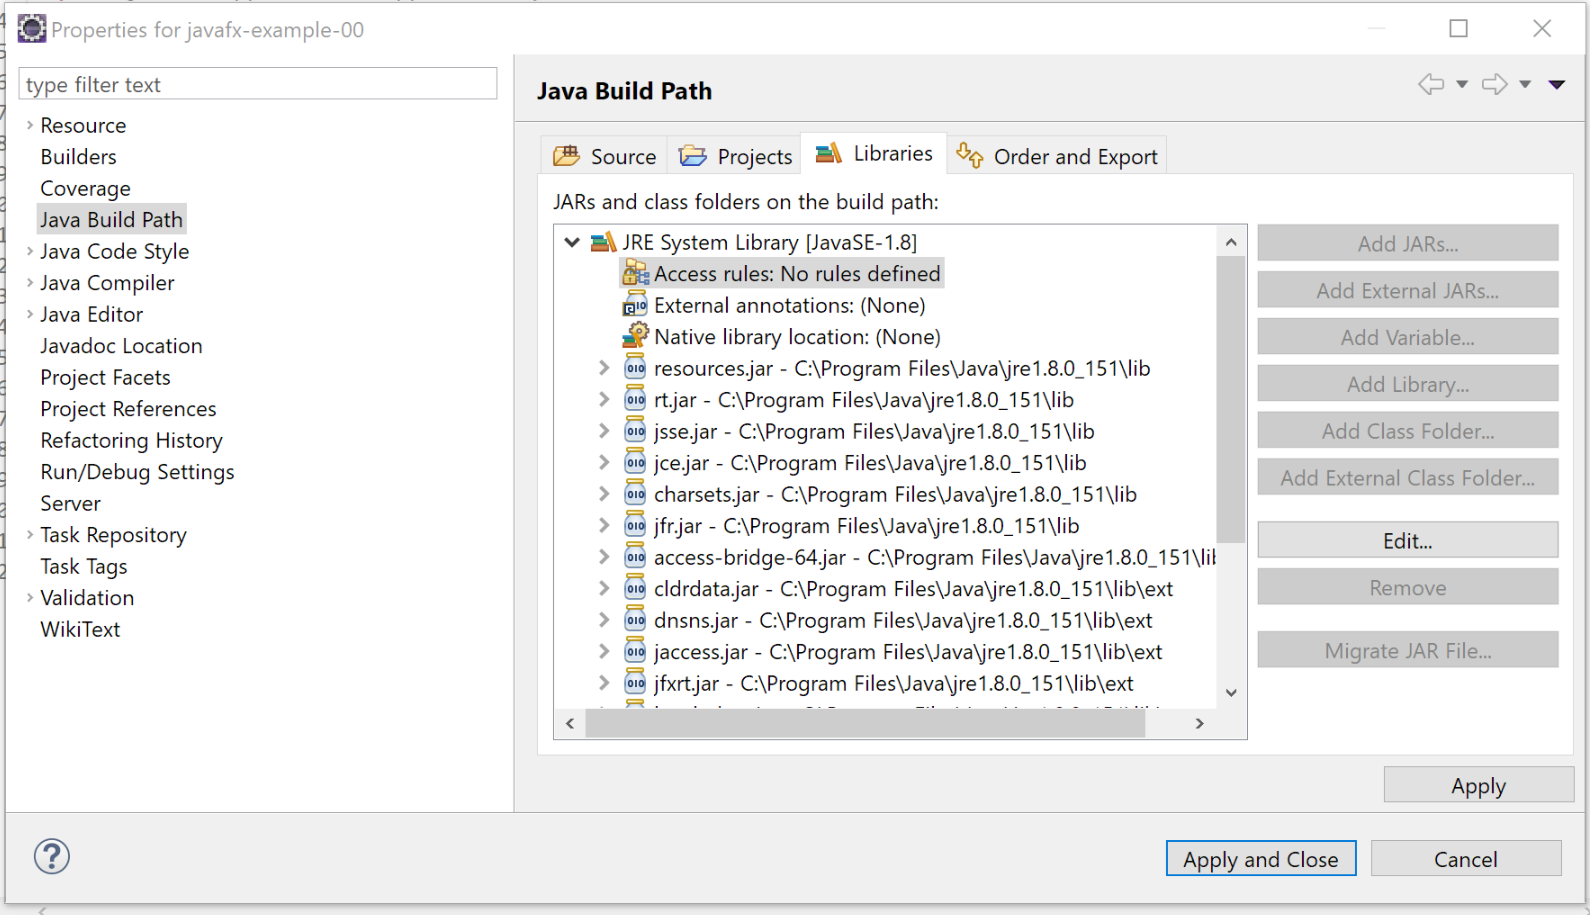
\includegraphics[width=0.9\textwidth]{img/conf01.png}
%\end{figure}
%\end{frame}
%
%\begin{frame}{Configurazione del progetto (2/2)}
%\begin{itemize}
%\item Click su Add $>$ Aggiungere una regola con:
%\begin{itemize}
%\item Resolution: \textbf{Accessible}
%\item Rule pattern: \textbf{javafx/**}
%\end{itemize}
%\item OK $>$ OK $>$ Apply and Close
%\end{itemize}
%\begin{figure}
%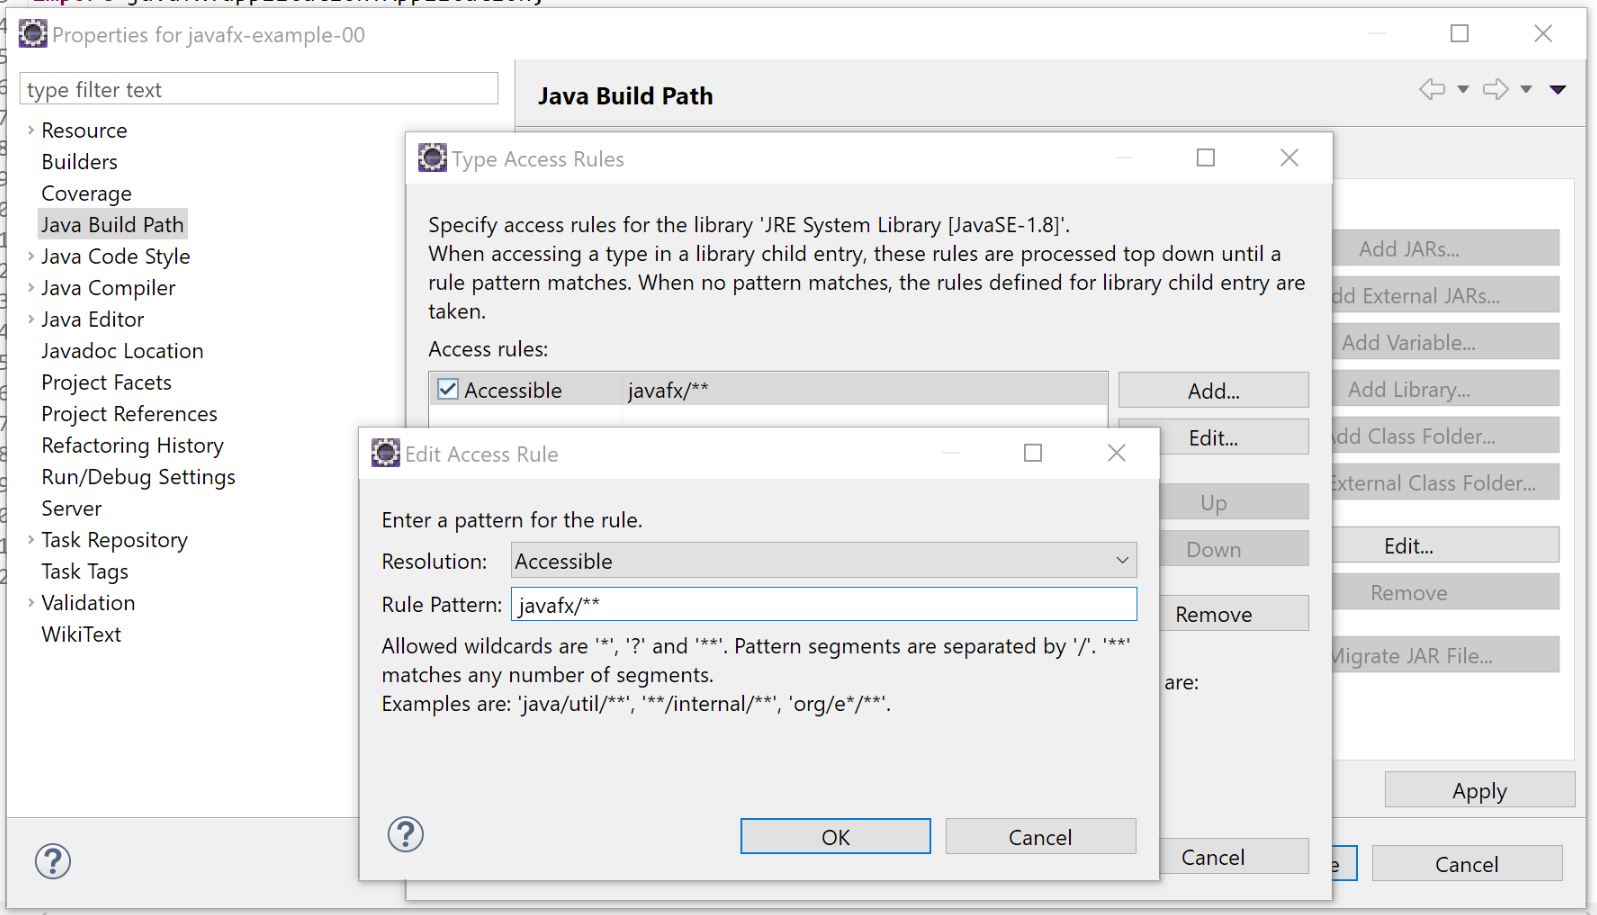
\includegraphics[width=0.85\textwidth]{img/conf02.png}
%\end{figure}
%\end{frame}

\subsection{Esecuzione di applicazioni JavaFX}

\begin{frame}{JavaFX in Eclipse}
\begin{itemize}\itemsep10pt
\item Da Java 11, JavaFX deve essere importato nel progetto come libreria esterna
\item Due alternative:
\begin{enumerate}
\item Si aggiungono tutti i JAR della libreria direttamente nel progetto
\begin{itemize}
\item Scaricabili da \url{https://gluonhq.com/products/javafx/}
\end{itemize}
\item Si specificano le dipendenze via \textbf{Gradle}
\end{enumerate}
\item Oggigiorno, è preferibile optare per la seconda alternativa
\end{itemize}
\end{frame}


\begin{frame}[fragile]{JavaFX e Gradle}
\begin{columns}[t]
\begin{column}{0.3\textwidth}
\begin{figure}
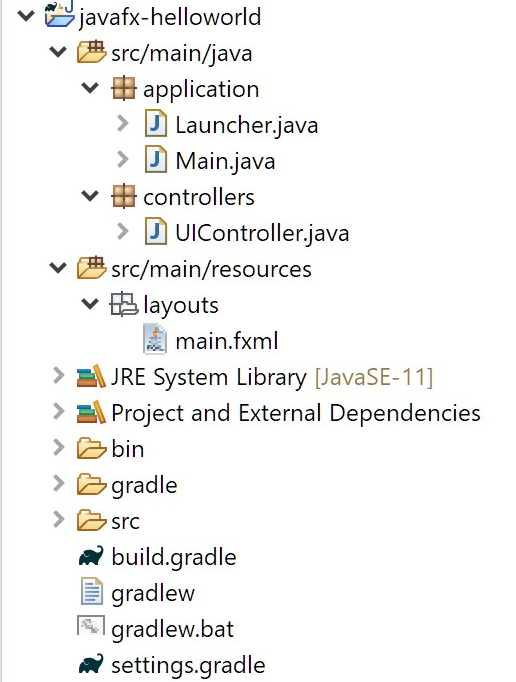
\includegraphics[width=\textwidth]{img/javafx-gradle-project.png}
\end{figure}
\end{column}
\begin{column}{0.7\textwidth}
\begin{block}{\texttt{build.gradle.kts} (sintassi Kotlin)}

\begin{lstlisting}[basicstyle=\tiny]
plugins {
    id("application")
    id("org.openjfx.javafxplugin") version "0.0.9"
}

repositories {
    mavenCentral()
}

javafx {
    version = "15"
    modules("javafx.controls", "javafx.fxml", "javafx.swing")
}

application {
  mainClassName = "application.Main"
}
\end{lstlisting}

\end{block}
\end{column}
\end{columns}
\end{frame}

\begin{frame}{Esecuzione dell'applicazione da Eclipse IDE}
\begin{itemize}\itemsep20pt
\item Si utilizza il task (predefinito) \emph{run} di Gradle -- accessibile dalla View \emph{Gradle Tasks} di Eclipse
\begin{figure}
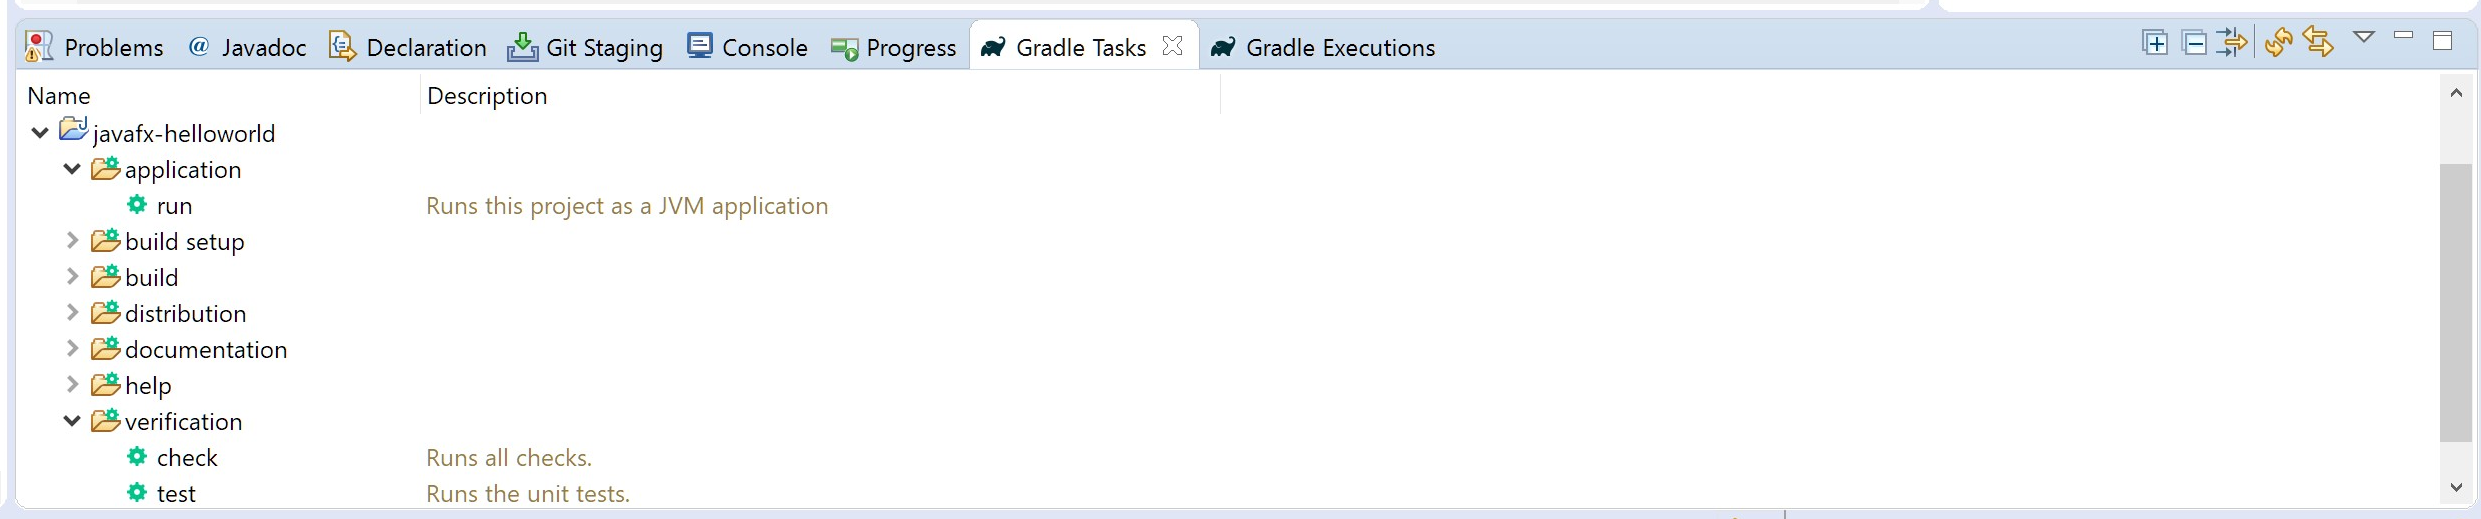
\includegraphics[width=0.9\textwidth]{img/gradle-tasks-view.png}
\end{figure}
\end{itemize}
\begin{itemize}
\item Qualora si voglia utilizzare il debugger, o eseguire l'applicazione in \emph{modo tradizionale}, è necessario specificare alcuni argomenti per la VM nella run configuration
\begin{itemize}
\item \texttt{--module-path \$\{project\_classpath:<PROJ-NAME>\}\\--add-modules javafx.controls,javafx.fxml}
\item Se JavaFX non è incluso tra le librerie del progetto, il percorso fornito a \texttt{--module-path} deve puntare alla cartella ove è presente l'SDK JavaFX
\end{itemize}
\end{itemize}
\end{frame}

\begin{frame}[fragile]{Generazione di JAR eseguibile per applicazione JavaFX}

\begin{itemize}
\item Si raccomanda l'uso di Gradle per la generazione di un ``fat JAR'', ovvero di un JAR che contiene al suo interno tutte le dipendenze necessarie a runtime
\item Occorre configurare il task \texttt{jar} come segue:
\begin{lstlisting}[basicstyle=\tiny]
// SINTASSI KOTLIN (build.gradle.kts)
tasks.withType<Jar> {
  manifest { attributes["Main-Class"] = "it.unibo.samplejavafx.App" }

  from(sourceSets.main.get().output)
    dependsOn(configurations.runtimeClasspath)
    from({
      configurations["runtimeClasspath"].map { if(it.isDirectory) it else zipTree(it) }
    })
}

// SINTASSI GROOVY (build.gralde)
jar {
    manifest { attributes 'Main-Class': 'myapp.Launcher' }
    from {
        configurations.runtimeClasspath.collect {
        	it.isDirectory() ? it : zipTree(it)
} } }
\end{lstlisting}
\end{itemize}
\end{frame}

\begin{frame}[fragile]{\texttt{build.gradle.kts} (completo -- sintassi Kotlin)}
\begin{lstlisting}[basicstyle=\tiny]
plugins {
  java
  application
  id("org.openjfx.javafxplugin") version "0.0.9"
}

repositories { jcenter() }

dependencies {
  /* for cross-platform jar: */
  runtimeOnly("org.openjfx:javafx-graphics:$javafx.version:linux")
}

javafx {
  version = "14"
  modules("javafx.controls", "javafx.fxml")
}

application.mainClassName = "application.Main"

tasks.withType<Jar> {
  manifest {
    attributes["Main-Class"] = "application.Main"
  }

  from(sourceSets.main.get().output)
    dependsOn(configurations.runtimeClasspath)
    from({
      configurations["runtimeClasspath"].map { if(it.isDirectory) it else zipTree(it) }
    })
}
\end{lstlisting}
\end{frame}


\begin{frame}[fragile]{\texttt{build.gradle} (completo -- sintassi Groovy)}
\begin{lstlisting}[basicstyle=\tiny]
plugins {
  id 'application'
  id 'org.openjfx.javafxplugin' version '0.0.9'
}

repositories {
  mavenCentral()
}

dependencies {
  /* for cross-platform jar: */
  runtimeOnly "org.openjfx:javafx-graphics:$javafx.version:win"
  runtimeOnly "org.openjfx:javafx-graphics:$javafx.version:linux"
  runtimeOnly "org.openjfx:javafx-graphics:$javafx.version:mac"
}

javafx {
  version = "14"
  modules = [ 'javafx.controls', 'javafx.fxml' ]
}

mainClassName = 'application.Main'

jar {
  manifest {
    attributes 'Main-Class': 'application.Main'
  }

  from {
    configurations.runtimeClasspath.collect { it.isDirectory() ? it : zipTree(it) }
  }
}
\end{lstlisting}
\end{frame}


\subsection{Scene Builder}

\begin{frame}{Scene Builder 2.0}
\begin{itemize}\itemsep10pt
\item Strumento per la creazione di GUI JavaFX-based in modalità drag-n-drop (GUI Builder)
\item Consente di esportare il file FXML relativo alla GUI disegnata
\item Distribuito come strumento esterno al JDK, non integrato (direttamente) in Eclipse
\item \url{https://gluonhq.com/products/scene-builder/}
\end{itemize}
\end{frame}

\begin{frame}{Scene Builder 2.0}
\begin{figure}
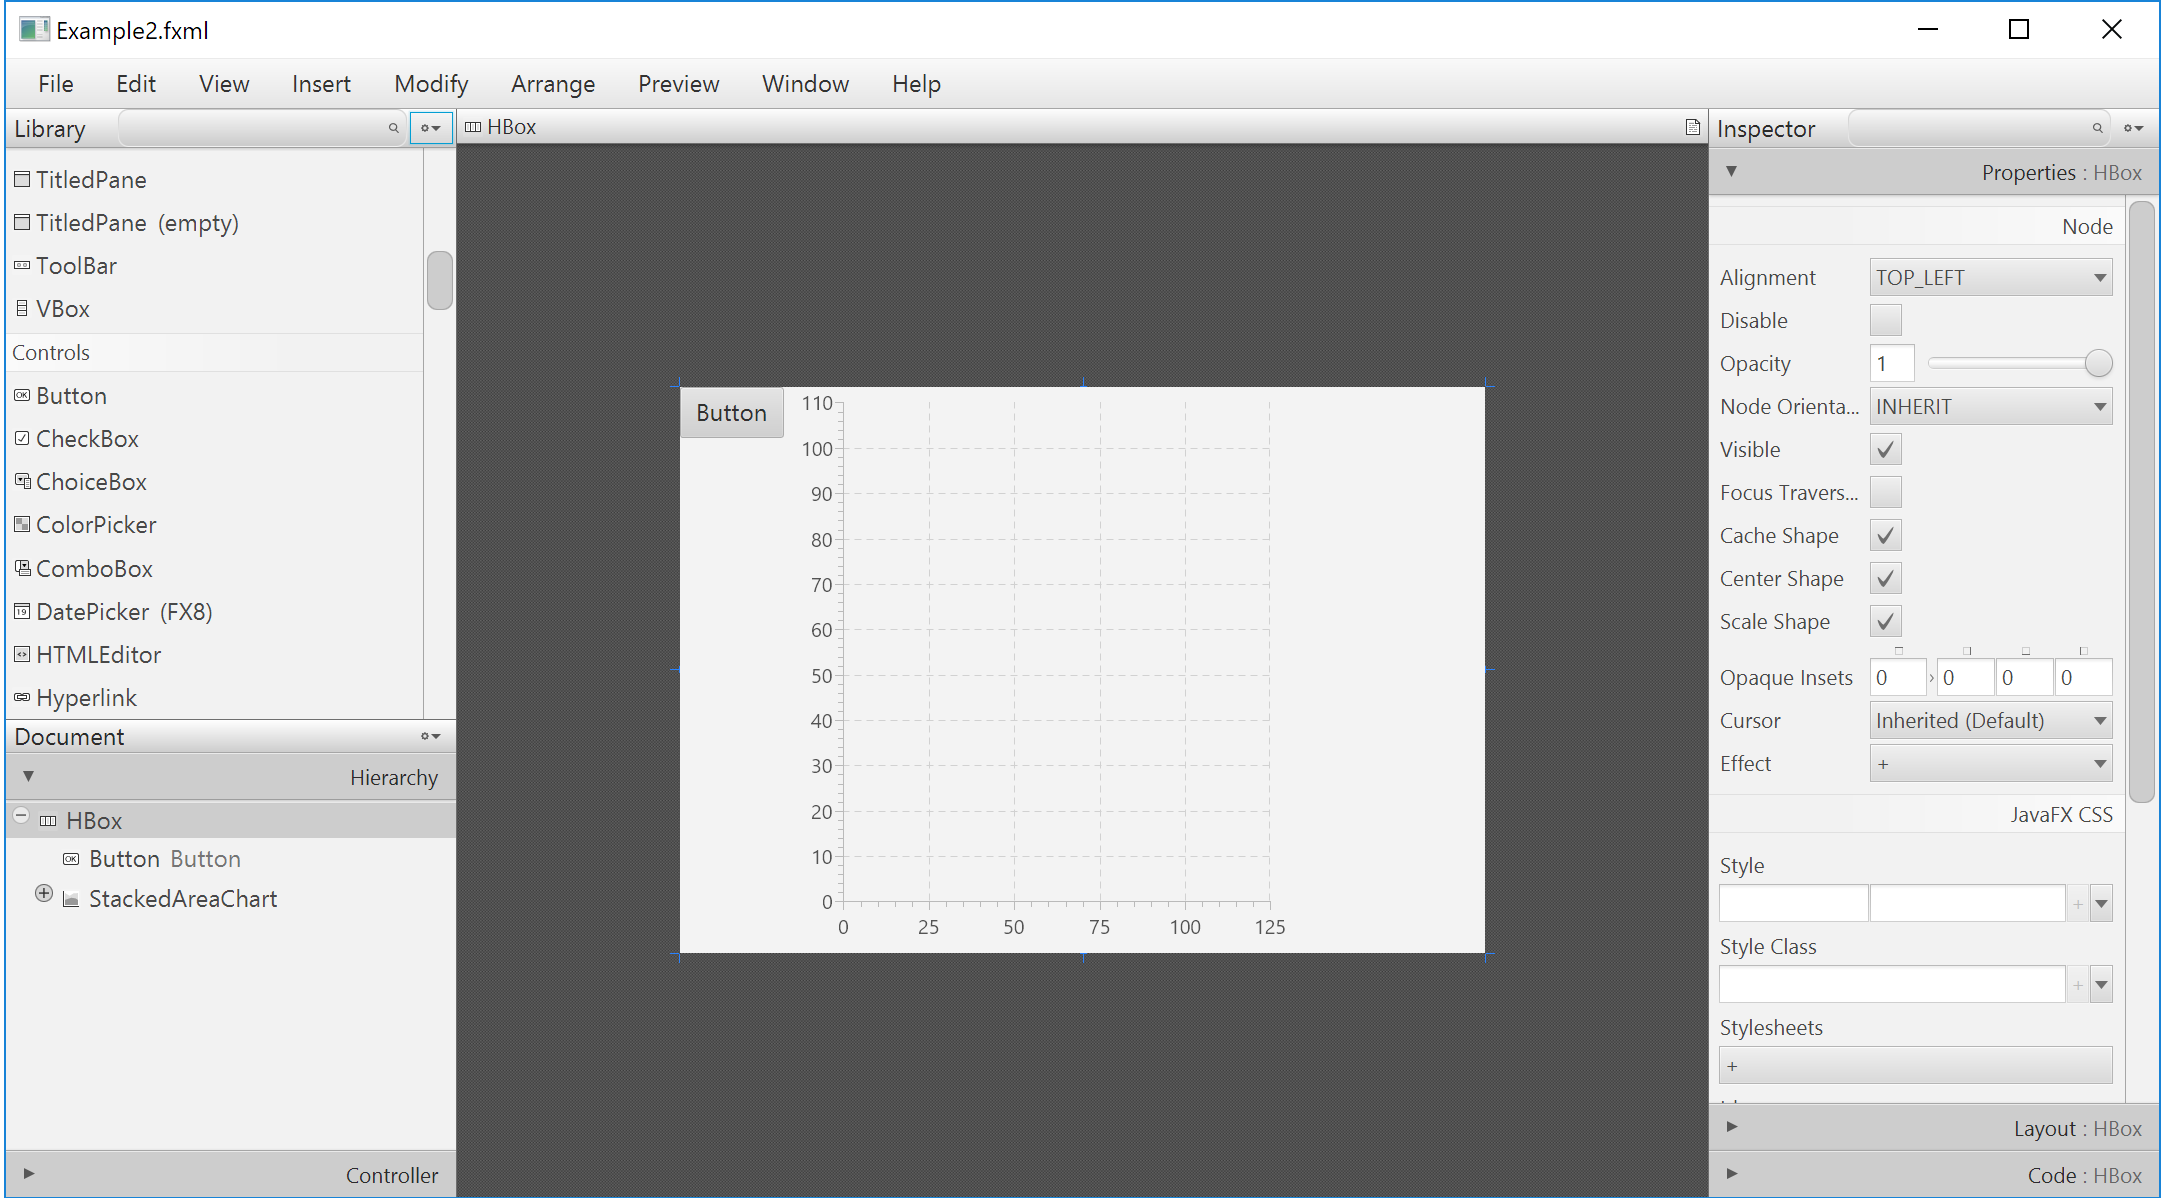
\includegraphics[width=\textwidth]{img/scenebuilder.png}
\end{figure}
\end{frame}

\subsection{Plugin e(fx)clipse}

\begin{frame}{Plugin e(fx)clipse}
\begin{figure}
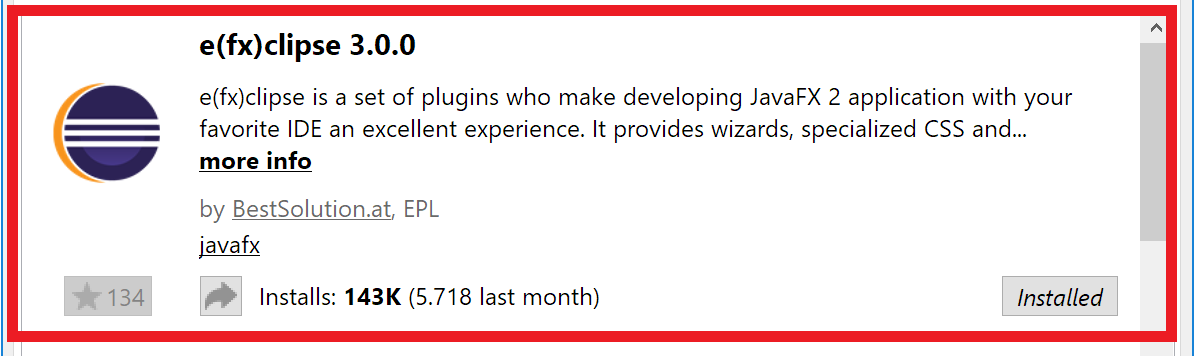
\includegraphics[width=0.76\textwidth]{img/plugin-install.png}
\end{figure}
\begin{itemize}\itemsep5pt
\item Plugin che fornisce una serie di tool per la gestione di applicazioni e progetti java basati su JavaFX
\item Consente di accedere al tool Scene Builder (installato separatamente) direttamente da Eclipse
	\begin{itemize}
	\item Configura da: \emph{Window $\to$ Preferences $\to$ JavaFX}
	\item Tasto dx su un file FXML $\to$ \emph{Open with SceneBuilder}
	\end{itemize}
\item Installabile dall'Eclipse Marketplace
\begin{itemize}
\item \url{http://www.eclipse.org/efxclipse/index.html}
\end{itemize}
\item \textbf{Va oltre le esigenze di questo corso...}
\end{itemize}
\end{frame}



%\begin{frame}[allowframebreaks]{Bibliography}
%\bibliography{biblio.bib}
%\end{frame}

\end{document}

